\documentclass{article}

\title{P02 Turing Machines Report}
\date{27/04/2018}
\author{150008859}

\setlength{\parskip}{1em}
\setlength{\parindent}{0em}

\usepackage{listings}
\usepackage{amsmath,amssymb,amsthm}
\usepackage{mathtools}
\usepackage{graphicx}
\usepackage{subfig}

\begin{document}
\maketitle
\newpage


\section{Introduction}


\section{Usage}

An ant build file is supplied. 

To compile the project, enter its directory. A build.xml file should be present. 

\begin{lstlisting}[language=bash]
  cd P02-Turingmachines
  ant clean
  ant compile
  ant jar
  ant run
\end{lstlisting}

\begin{figure}[!htb]
  \caption{The file dialog, please select a machine}
  \centering
  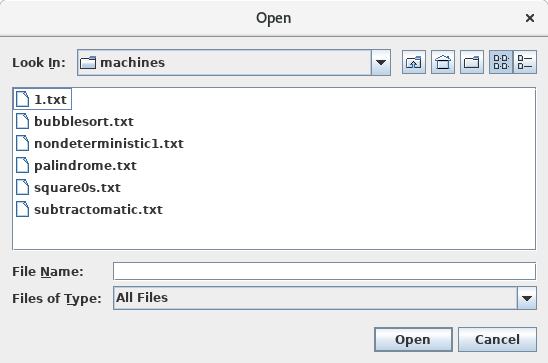
\includegraphics[scale=0.30]{images/filedialog.png}
\end{figure}

\begin{figure}[!htb]
  \caption{The graphical user interface}
  \centering
  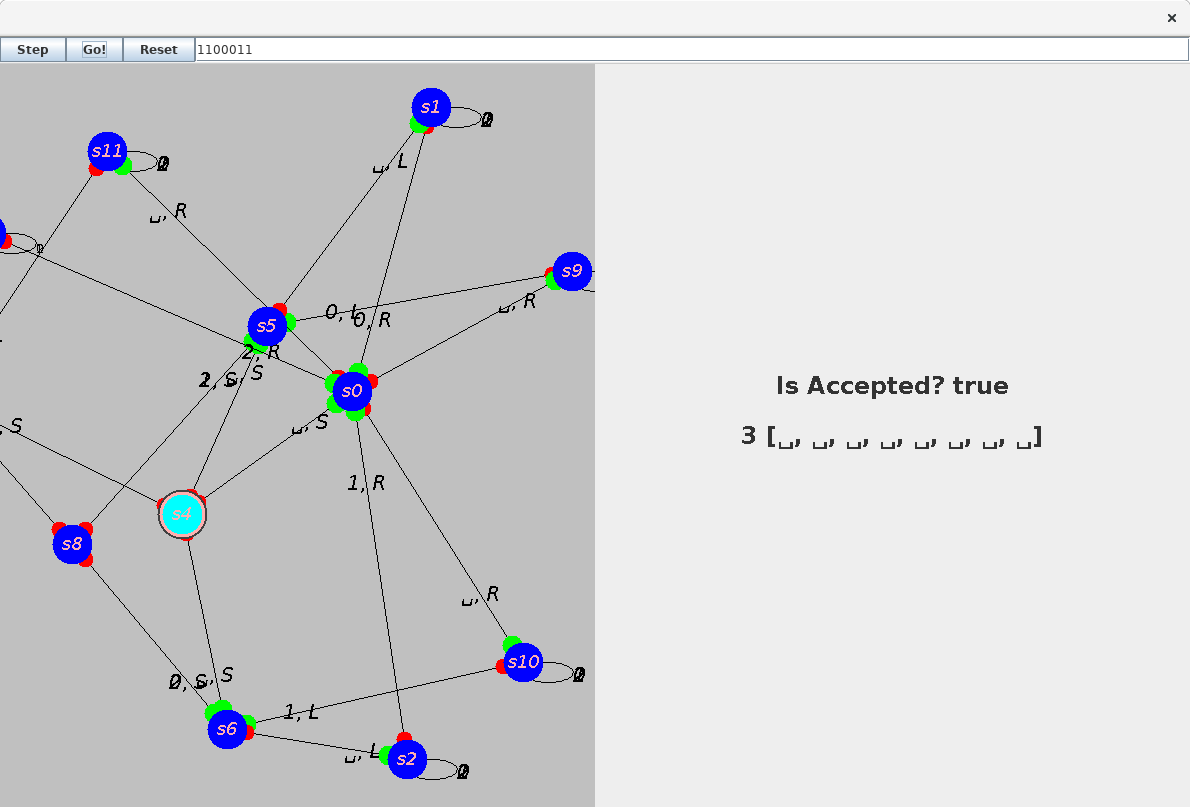
\includegraphics[scale=0.15]{images/gui1.png}
\end{figure}


Running the project, the user is presented with a file dialog. Select a file in the ``machines'' folder e.g. ``palindromes.txt''

The user is now presented with a graphical user interface.

Press \textbf{reset} to load the string present in textbox at the top into the tape.

Pressing \textbf{step} takes a single step.

Pressing \textbf{Go} resumes play until the halting state is reached, reset cancels this operation.

All turing machine programs can be found in the ``machines'' folder.

If there is trouble using the ant build system, the project itself is an eclipse project with the main method in ``turing.gui.UserInterface''.

Reproducing the experiment would involve opening the project as an eclipse project and running the main method present in ``turing.experiment.Data''.  To reproduce the graphs for the experiment, enter the ``experiment'' directory and run the ``python3 experiment.py''. All the results are found present in that directory as well.

\section{Tasks Accomplished}

\begin{itemize}
\item (Task 1) Turing Machine Simulator which accepts the suggested input. 
\item (Task 2) 
  \begin{enumerate}
  \item Recognise palindromes.
  \item Recognise strings from the language $ \{ w_1\#w_2\#w_3 \mid w_3 = w_1 + w_2 \} $
  \item Bubble Sort
  \item Recognise strings of the form $0^{2^n}, n \geq 0$
  \end{enumerate}
\item (Task 3) Analysis of all turing machines.
\item (Task 4) Implement Non-deterministic turing machine and attempt at solution.
\item (Extension) Graph drawing and visualisation.
\item (Extension) Turing machine state and tape visualisation.
\item (Extension) Graphical User Interface.
  
\end{itemize}

\section{Task 1}

A turing machine simulator is provided which accepts the suggested input. The input is parsed. A hashset is used to store all the states, another hashset stores all the accepting states. Each state (Stt.java) contains a function named delta, when given an input symbol (Sym.java), it returns a list of three tuple (Out.java) which consists of the replacement symbol, the direction to move and the next state to move to. The delta function uses a hashmap which maps the input symbol to a list of Outs. Ordinarily, the list of Outs contains one element for each input, unless non-determinism is involved in which case it have multiple. The null key in the hashmap is reserved to store epsilon transitions.

\section{Task 2}

\subsection{Recognise palindromes}

\begin{figure}[!htb]
  \caption{A turing machine to recognise palindromes.}
  \centering
  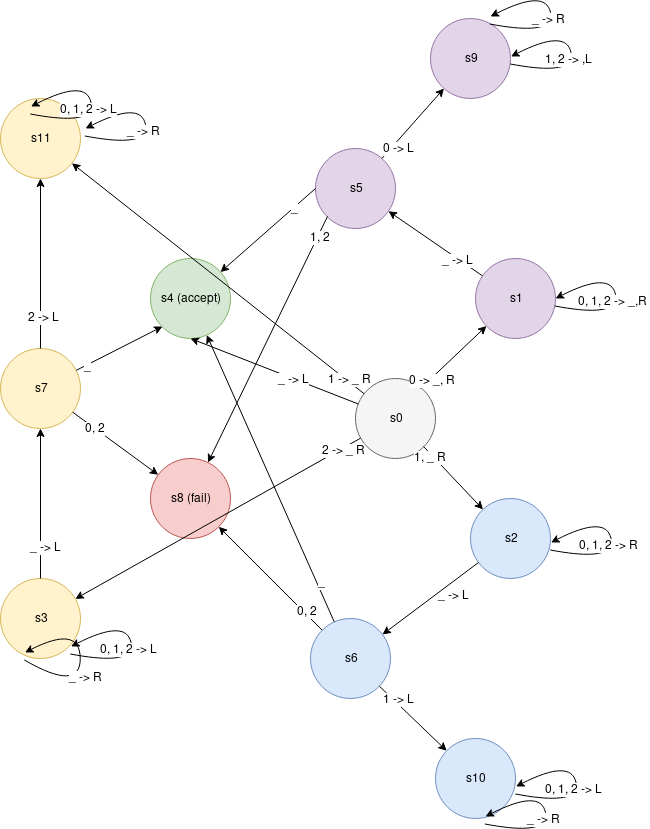
\includegraphics[scale=0.30]{images/palindrome.png}
\end{figure}

The algorithm then checks the first number, enters the set of states that signify it has seen that particular number (signified by the different colours in the diagram). It crosses that number off, it then moves all the way to the right. If that number is identical it will move back to the first state causing it to move back and the process to repeat. However, if the number is not identical, it will enter the rejection state. All the numbers have been compared when in state 1 and moving back right encounters a blank space immediately and the machine can proceed into the accepting state.

\newpage

\subsection{Recognise strings from the language $ \{ w_1\#w_2\#w_3 \mid w_3 = w_1 + w_2 \} $}

\begin{figure}[!htb]
  \caption{A turing machine to recognise $ \{ w_1\#w_2\#w_3 \mid w_3 = w_1 + w_2 \} $}
  \centering
  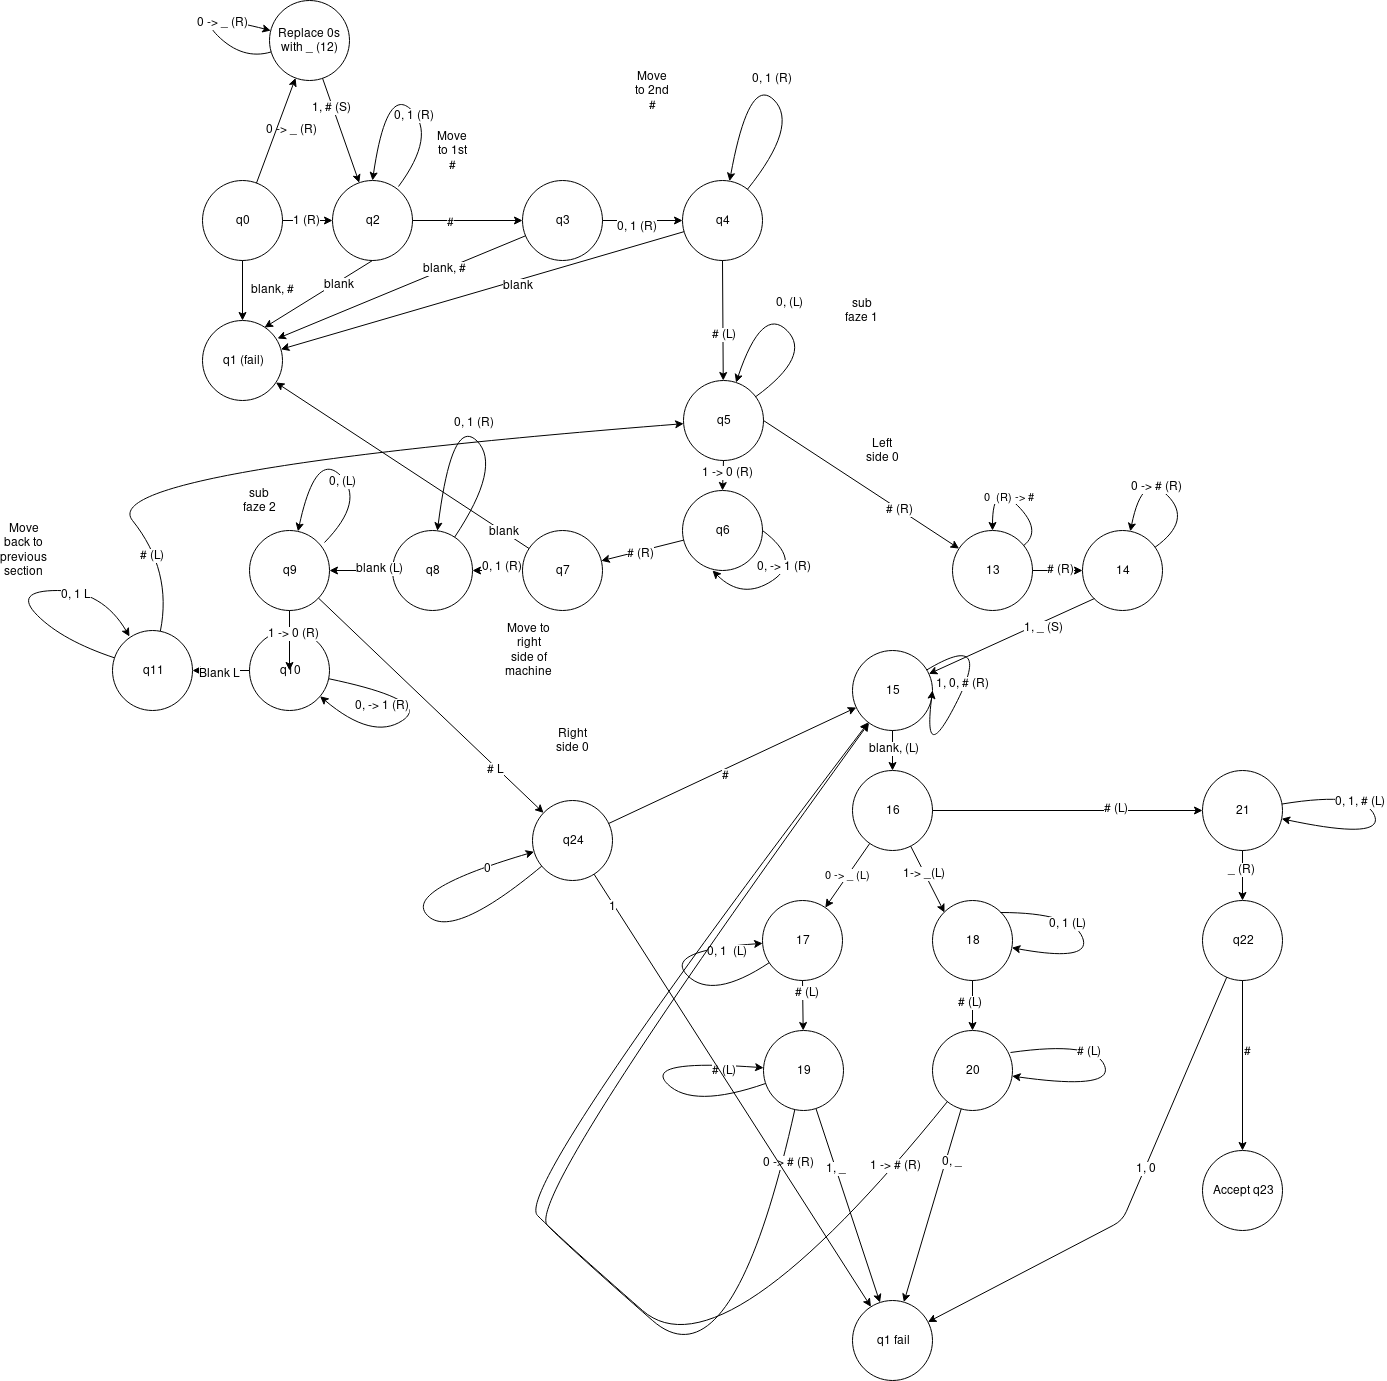
\includegraphics[scale=0.20]{images/subtractomatic.png}
\end{figure}

I accidently ignored the part of the question where you can assume $w_3$ is in lsb first order. Hence, this program works with $w_3$ with msb first order.

The algorithm begins by subtracting from $w_3$ and $w_2$ until one of them reaches 0.

If $w_2$ reaches 0, then you check if $w_1$ and $w_3$ are equal and in which case we accept or otherwise reject, the most significant 0 bits are removed by padding them with $\#$ or blanks to allow this to happen.

If $w_3$ reaches 0, then check if $w_2$ is 0. If $w_2$ is not zero, then fail as $w_2$ is greater than $w_1$. Otherwise, we can use the previous comparison set of states to check if $w_1$ and $w_3$ are equal in which case we accept or otherwise reject.

\newpage

\subsection{Bubble Sort}

\begin{figure}[!htb]
  \caption{A turing machine to perform bubble sort.}
  \centering
  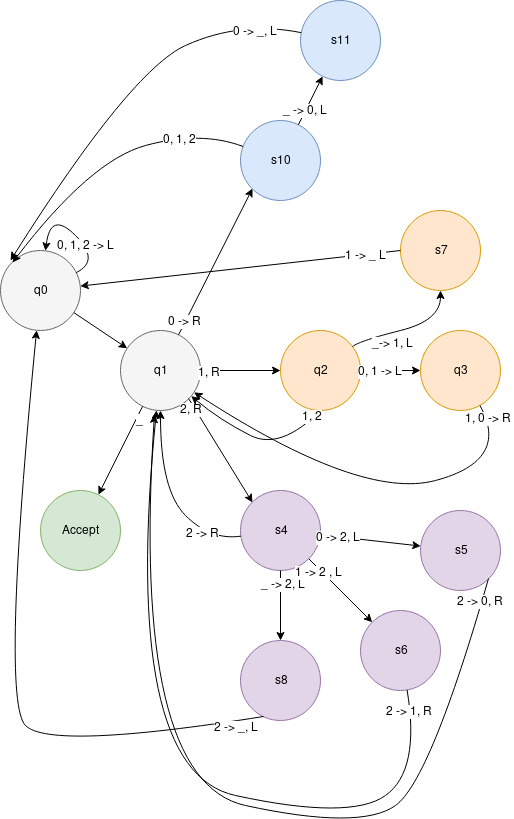
\includegraphics[scale=0.30]{images/bubble.png}
\end{figure}


The bubble sort algorithm iterates from left to right, forming a bubble between pairs as it moves. If the first element in the pair is bigger than the second element, then they are swapped. This causes the largest item to move all the way to the front of the list. The blank space is used as a divider at the end to seperate the sorted list from the unsorted list. This causes the number of iterations to decrease by 1 each time. The sorting algorithm terminates once the divider reaches the start of the list. The comparison is encoded in set of states entered by the choice of the first number, this is color coded on the diagram.


\newpage

\subsection{Recognise strings of the form $0^{2^n}, n \geq 0$}

\begin{figure}[!htb]
  \caption{A turing machine to recognise $0^{2^n}, n \geq 0$}
  \centering
  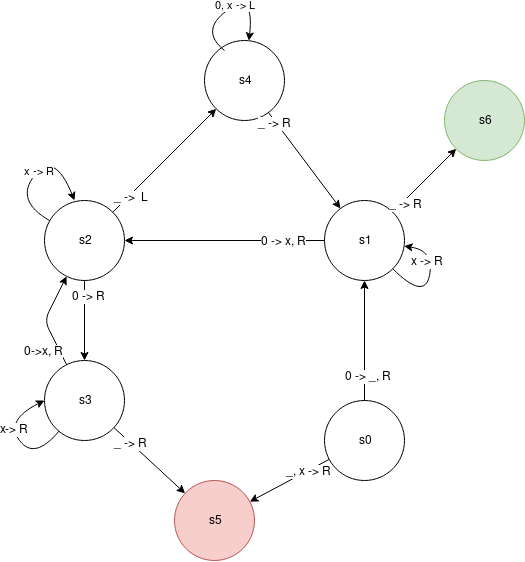
\includegraphics[scale=0.30]{images/square0s.png}
\end{figure}


I selected this algorithm from Sipser as it was one of the first turing machine algorithms I encountered while learning about turing machines. The machine iterates through the tape while eliminating every other 0s cutting the number 0s to half. If the number of 0s seen is not one, but odd then we can reject as the only square number that fits this category is 1. However, If the number of 0s seen is 1, then we accept. For example for the number 8, it would be broken down into 8, 4, 2, 1 at which point it would be accepted.


\section{Task 3}

\subsection{Palindrome}

\begin{figure}[!htb]
  \caption{}
  \centering
  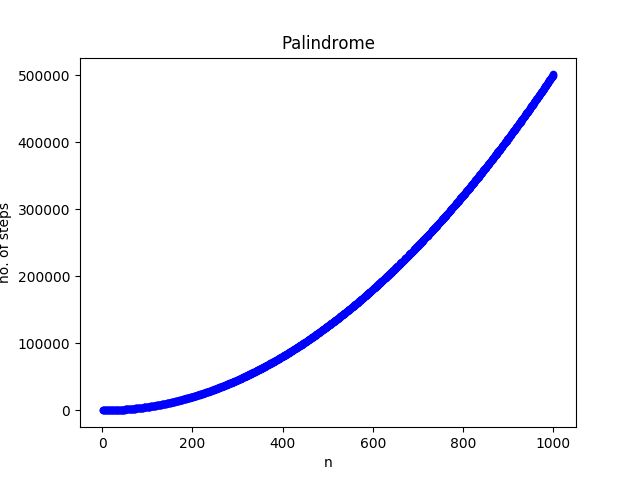
\includegraphics[scale=0.50]{images/palindrome_graph.png}
\end{figure}

There are n steps taken when moving all the way from right to left, this decreases by 1 each iteration. There are also n steps involved while moving back all the way to the left and this decreases by 1 each iteration. In addition, there are n iterations. Hence, we can use double the $ S_n $ formula to calculate the number of steps. The number of operations is $ 2 \cdot \frac{1}{2} \cdot n (n+1) = n (n + 1)$ as a function input size. This function is $O(n^2)$.

\subsection{Subtractomatic}

\begin{figure}[!htb]
  \caption{}
  \centering
  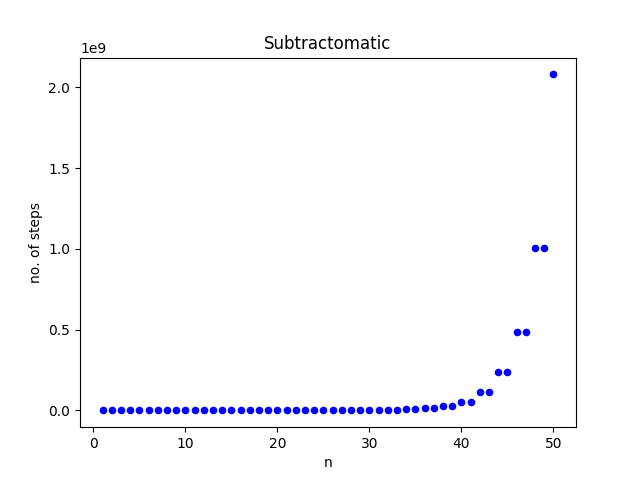
\includegraphics[scale=0.50]{images/subtractomatic_graph.png}
\end{figure}

1 is subtracted from the number each step. Subtracting 1 from a number in base 2 for a number of length n in the worst case scenario where all of the digits are 1 takes $2^n - 1$ steps. This is exponential time complexity and is $O(2^n)$. The other step where the first part of the string is compared to the end part of the string is $O(n^2)$ due to the sum of 1 to n formula. However since $O(2^n)$ is much larger than $O(n^2)$ as n tends to infinity, we can ignore the latter term. Hence, the time complexity $O(2^n)$.

\subsection{Bubble Sort}

\begin{figure}[!htb]
  \caption{}
  \centering
  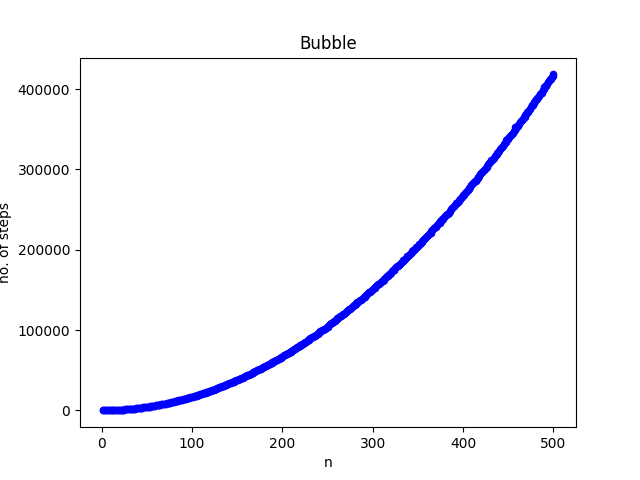
\includegraphics[scale=0.50]{images/bubble_graph.png}
\end{figure}

Bubble sort iterates from left to right, this is decreased by 1 each iteration. There are n steps involve when returning to the start. Hence, for the same reasons as the palindrome doubling the $S_n$ formula produces $ n (n + 1) $ which is $O(n^2)$.

\subsection{Square number of 0s}

\begin{figure}[!htb]
  \caption{}
  \centering
  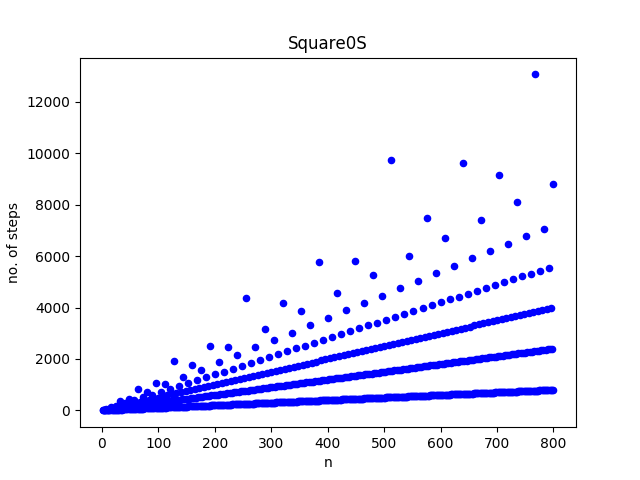
\includegraphics[scale=0.50]{images/square0s_graph.png}
\end{figure}

This produces the most interesting graph out of all of the result. The worst scenario is when the number of 0s is square. In this case, the machine must iterate back and forth while halving the number of 0s until there is only 1 left. The number of times this must happen is $log_2(n)$. For each of these halvings, the machine iterates forward, backwards which is $2 \cdot n$ times. Hence, the time complexity is the product $2 \cdot n log_2(n) $ which is $O(nlog_2(n))$.

\section{Task 4}

I implemented non determinism. A list of ``mini machines'' execute concurrently. When multiple transitions are defined for the same input, the original machine is deleted and a child machine is created for every transition and added to this list. Epsilon transitions are also handled, in this case the parent is not deleted. Epsilon transitions are followed until there are no more epsilon transitions that can be followed. If there was a cycle of epsilon transitions, the program would be stuck in an infinite loop. Halted machines which are not in an accepted state are pruned. The turing machine enters the accepted state if one of the ``mini machines'' is halted and its current state is in the set of accepted states.

Input of the following form will create non deterministic turing machines.

\begin{lstlisting}[language=bash]
  s0 a s1 a R
  s0 a s2 a R
\end{lstlisting}

It accepts epsilon transitions in the following manner.

\begin{lstlisting}[language=bash]
  s3 epsilon s6
  s6 epsilon s0
\end{lstlisting}

I created one example to demonstrate it works, the program can be found in ``nondeterministic.txt'', give it the input of ``aaaaa''. The machine itself is nonsensical, but it highlights the fact that the non-determinism works.

\begin{figure}[!htb]
  \caption{Demonstrating non-determinism}
  \centering
  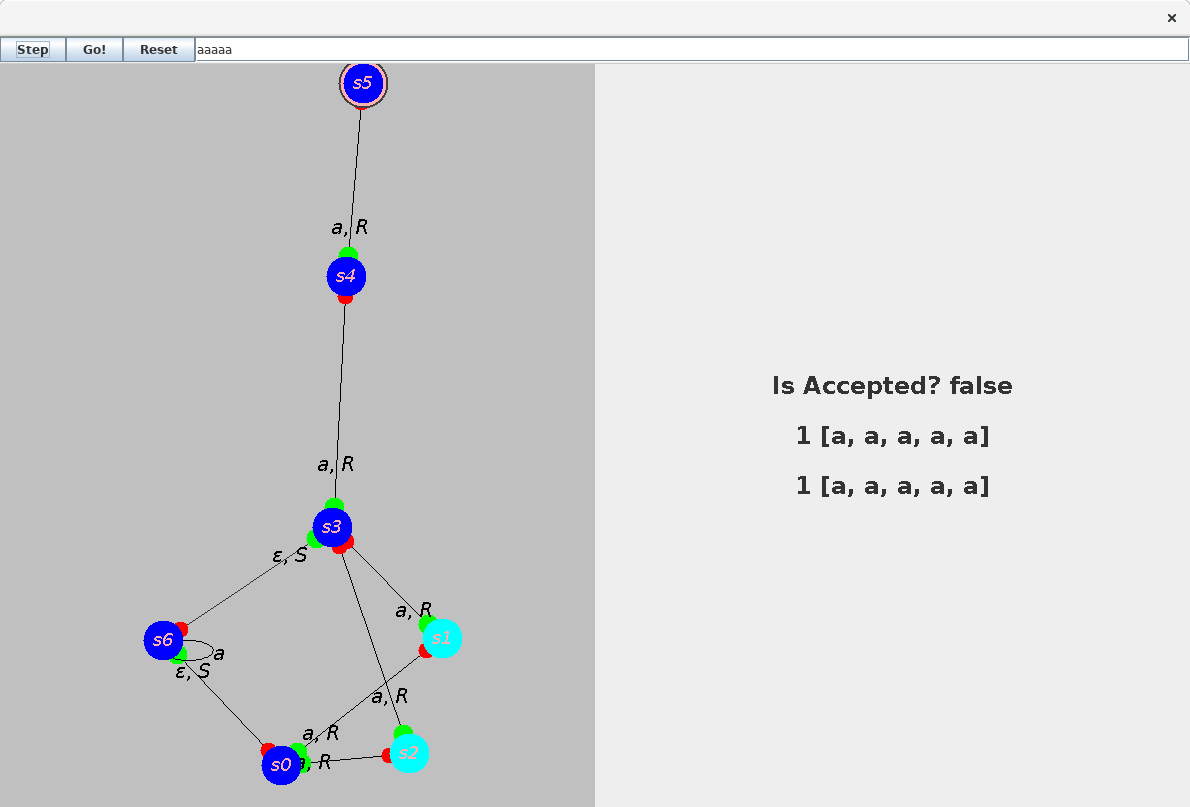
\includegraphics[scale=0.13]{images/nondeterminism.png}
\end{figure}

\subsection{Non-deterministic palindrome}

I could not think of a solution to the non deterministic palindrome solution using turing machines. However, after some research, this problem can be solved using non deterministic push down automata. The issue with non deterministic automata is that you want to push half of the input on and then pop it while it comparing it to the other half. However, it is not easy to determine where the center of the string is. With a non deterministic push down automata you can guess you have reached the middle of the string at every position and split the machine into two children. One child assumes it has reached the center, the other one doesn't and proceeds to move through. The one that proceeds to move through continues to splits into two. If the guess was correct, then the machine produced by that enters will the accepting state.

\section{Extensions}

I used the force directed placement graph drawing algorithm \cite{forcedirected} in which attractive ``forces'' are applied between edges and repulsive ``forces'' between nodes. This is used to display the states of the turing machine. As the turing machine runs, the current state is highlighted. The end state is highlighted different from all the states.

\section{Evaluation}

I really enjoyed this practical, tried my best and started very early, however I feel as if I wasn't able to accomplish everything I wanted, document some of the more interesting parts of practical or document things in more detail due to time constraints caused by the JH project. 

\begin{thebibliography}{1}
  
\bibitem{forcedirected}
Fruchterman, Thomas MJ, and Edward M. Reingold. "Graph drawing by force‐directed placement." Software: Practice and experience 21.11 (1991): 1129-1164.

\end{thebibliography}

\end{document}
